
\documentclass[12pt, a4paper, oneside] {book}
\usepackage[english]{babel}
\usepackage[utf8]{inputenc}
\usepackage[T1]{fontenc}

\usepackage{subfig}
\usepackage{xcolor}
\usepackage{url}
\usepackage{fancybox, graphicx}
\usepackage{tikz}
\usetikzlibrary{shadows}
% \usepackage{fancyhdr}
% \usepackage{setspace}

\usepackage{ae,aecompl}
% \usepackage{amsfonts}

% \usepackage{array}
% \usepackage{stmaryrd}
% \usepackage{algorithmic}

% \usepackage{url}

%Javascript

\begin{document}

%\pdfbookmark{Title}{Title}
\begin{titlepage}

\begin{center}

\begin{LARGE}\textbf{\sc University of Pisa}\end{LARGE}\\
\vspace{0.3cm}
\begin{LARGE}\textbf{\sc Scuola Superiore Sant'Anna}\end{LARGE}

\vspace{2.0cm}

\includegraphics[scale=0.4]{cherubino.png}
\hspace{1.0cm}
\includegraphics[scale=0.74]{sssup.png}

\vspace{1.0cm}

\begin{Large}
\sc Department of Computer Science\\
\sc Department of Information Engineering\\
\vspace{0.28cm}
\sc And Scuola Superiore Sant'Anna
\end{Large}

\vspace{0.8cm}

\large MASTER DEGREE ON COMPUTER SCIENCE AND NETWORKING\\
(Class LM-18)

\vspace{1.4cm}

{\bfseries \LARGE Distributed Enabling Platform Project}\\[0.3cm]
{\sc \Large Distributed File System}\\[1.7cm]

\begin{LARGE}
Stefano Ceccotti 456568\\
\end{LARGE}

\vspace{0.32cm}

\begin{large}
Accademic Year 2015/2016
\end{large}

\end{center}

\end{titlepage}

\tableofcontents

\chapter{Introduction}

The project of Distributed Enabling Platform consists in creating an eventually consistent Distributed File System.
The system provides simple operations to work with it:

\begin{itemize}
  \item \textbf{get}: to retrieve a file from the system;
  \item \textbf{put}: to store a file in the system;
  \item \textbf{delete}: to remove a file in the system;
  \item \textbf{getAll}: to retrieve all the files stored in a random node.
\end{itemize}

The system makes use of Gossiping, Versioning (namely Vector Clock), hinted handoff, Anti-Entropy and Consensus (a.k.a. Quorum) protocol.
The Anti-Entropy mechanism ensure that the system, if no new updates are made to a given data item, eventually all accesses to that item will return the last updated value
(from here the eventual consistency).\\
Using hinted handoff, we ensure that the read and write operations are not failed due to temporary node or network failures.

\chapter{System Architecture}

The project is composed of 3 entities: \textbf{Client}, \textbf{LoadBalancer} and \textbf{StorageNode}, arranged in the following way:\\

\begin{figure}[!htpb]
\centering
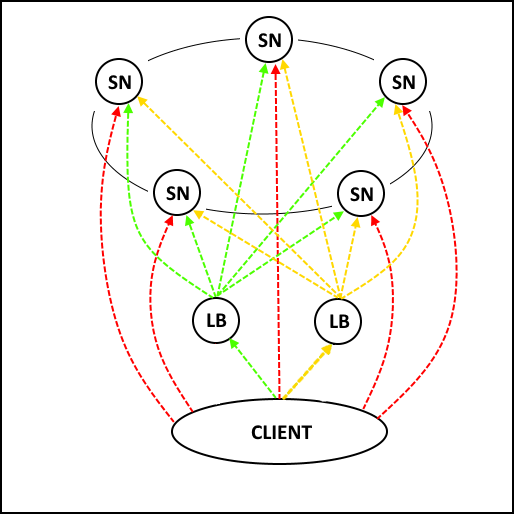
\includegraphics[width = 120mm, height = 90mm]{img/system.png}
\caption{Abstract version of the system. The green and yellow dashed lines are possible paths that a request may follow when
the client uses \textbf{LoadBalancer}s, while the red dashed ones are direct connections to the \textbf{StorageNode}s.}
\label{fig:abstract_orchestration}
\end{figure}

\begin{itemize}
  \item \textbf{Client}: interacts with the user and transmits the message requests;
  \item \textbf{LoadBalancer}: receives the client requests and forwards them to the correct node based on the their workload;
  \item \textbf{StorageNode}: receives requests either from load balancers or directly from clients. It also provides a way to store the files in a consistent manner.
\end{itemize}

All the connections use TCP in order to have a reliable mechanism, especially when files are transferred,
at the cost of a little overhead due to the connection establishment.
Every connection has a timeout of 2 seconds (except from StorageNode to Client that are 5 seconds), after that, if it has not been established,
means that the destination node is dead or something wrong happened.


\section{StorageNode}

The StorageNode is the entity used to store the files received by client requests.
Everytime a new request arrives, a new Thread is activated (from a fixed ThreadPool) and a TCP connection is open: if the request arrives from a load balancer, then a direct TCP connection
is opened with the client, closing the initial one. This is done to reduce the workload on the load balancers, and to eliminate the triangular problem, similar to Mobile IP \cite{rif1}.\\

\begin{figure}[!htpb]
\centering
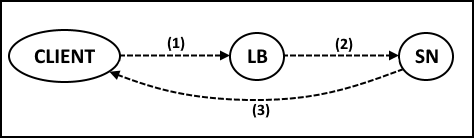
\includegraphics[width = 115mm, height = 32mm]{img/communication.png}
\caption{Communication pattern.}
\label{fig:abstract_orchestration}
\end{figure}

The logical structure of the node is the following:

\begin{itemize}
  \item \textbf{MembershipManagerThread}: Thread responsible to receive the membership requests from a client;
  \item \textbf{QuorumThread}: Thread responsible to perform the quorum protocol;
  \item \textbf{AntiEntropyThread}: Thread responsible to perform the anti-entropy mechanism;
  \item \textbf{MonitorThread}: Thread used to monitor the state of StorageNode instances;
  \item \textbf{NetworkMonitorThread}: Thread used to send informations about the own workload;
  \item \textbf{DFSDatabase}: Class used to manage the files stored on it.
\end{itemize}
Every StorageNode is in charge of all the keys whose id is less or equal than the node's one.
The node id is computed applying the SHA-1 hash function to its Ip address and the virtual node instance, while for the files only on their name.\\
The virtual node mechanism is a technique used to distribute, in a more uniform way, the nodes inside the DHT using the so called ``tokens'' as a logical replication of
a phisical node. Instead of a ``per-instance'' value, the number of available tokens is computed using the capability of the machine.

\subsection{Storage System}

All the files are stored using a B-Tree structure to efficiently put, get and delete files in memory and on disk as well.
Each file can be accessed simultaneously only in read mode, otherwise (write mode) in a mutually exclusive way \cite{rif2}.\\
To reduce the latency inside the operations, due to the access on disk, an \textbf{AsyncDiskWriter} Thread is enabled by default.
In this way all the modifications are performed in asynchronous mode and do not block.\\
It is possible to disable the Thread, but this greatly hurts concurrency. Without async writes, all threads remain blocked until all previous writes are not finished (single big lock).

Along with data it is associated a \textbf{VectorClock}, that keeps track of all the nodes that have updated the file.
A VectorClock is effectively a List of (node, counter) pairs, where the counter is increased by one by the Coordinator node (the node in charge of the key).
If more than 10 versions of the file are present, the one with the oldest timestamp is discarded.

%One can determine whether two versions of an object are on parallel branches or have a causal ordering, by examine their vector clocks.
%If the counters on the first object’s clock are less-than-or-equal to all of the nodes in the second clock, then the first is an ancestor of the second and
%can be forgotten. Otherwise, the two changes are considered to be in conflict and require reconciliation.

When a file is added or removed its hinted handoff value is checked: if different from \emph{null} the file will be stored also in a different database inside the \textbf{HintedHandoffThread}:
this Thread saves all the files associated to a specific destination node and, periodically (every 60 seconds), tries to send the associated files:
once the transfer succeeds, the files will be removed from its local store without decreasing the total number of replicas in the system.

\subsection{Quorum Protocol}

If a node receives a GET\_ALL request then it simply returns all the files stored in its database, otherwise a quorum mechanism is started; this node is the previously defined Coordinator node.
If the quorum is reached the requested operation is performed, otherwise a negative response is returned to the client.\\
The quorum can be reached only if N/2+1 of the contacted nodes agree to it, for both read and write requests.
The quorum request is managed by a Background Thread called \textbf{QuorumThread},
which contains a HashMap of (String, QuorumFile) to efficiently checks if the requested file is locked or not.
In addition, a unique identifier is associated to each request to prevent some mistakes due to reordered commits: requests with an id different than the expected one are discarded.

When a file is locked, the Thread waits for the Commit request: when it is received, and the id is the expected one, the file is unlocked.
This mechanism ensure that each file can be accessed in an exclusive way by the node that has sent the request. Simultaneous accesses are allowed only for files accessed in read mode.\\
This approach is called Two-phase commit protocol \cite{rif3}, but with a small variance:
to alleviate deadlock situations, due to some error in the Coordinator node, each file mantains the locking state for a maximum of 60 seconds, after that the file is unlocked.

\subsection{Anti-Entropy Mechanism}

The anti-entropy mechanism is a background task used to resolve possible inconsistencies between files owned by different nodes.
It's performed by means of a \textbf{Merkle tree} structure, which consists in a tree of hashes (tipically MD5) in which the leaves are hashes of a set of files (in this implementation the name of the file).
Every level is the hash function applied to the concatenation of their respective children.\\
The \textbf{AntiEntropySenderThread} and \textbf{AntiEntropyReceiverThread} are the two classes used to perform the anti-entropy protocol.
The sender only transmits the Merkle tree level, while the receiver only returns a response.
It's articolated in 4 phases, executed periodically:

\begin{itemize}
  \item [\textbf{1.}] \textbf{Node choosing}: the sender node exchange the own Merkle tree with the succesor node encountered in the DHT, to retrieve the keys managed by requestor node,
					      and with a random node among the N predecessor ones, to control if there is any difference between the ``original'' and the own replica files;
  \item [\textbf{2.}] \textbf{Handshake}: the sender node sends the range of the considered keys and the height of the own tree. The latter value is important to reduce the cost of the operation,
					  because in case the trees have different levels the highest one is reduced to reach the other level, since the hash of nodes belonging to different levels are
					  obviously differents;
  \item [\textbf{3.}] \textbf{Merkle tree exchange}: the sender node sends the current level (typically starting from the root), then the receiver compares it with the own current one:
						     if equals, the operation is stopped, otherwise the children of the different nodes are sent and compared,
						     repeating this operation until the leaves are reached.
						     If two nodes are equals a bit is set to 1 to all the leaves reached by that node, using a specific BitSet object;
  \item [\textbf{4.}] \textbf{Version exchange}: in case of common files (at least one bit set to 1) the sender node sends a list of VectorClock, one for each common file,
						 to verify if the version of the file owned by the sender is the most updated one.\\
						 So the receiver sends, in addition to the all non-common files, all the files younger than the received ones.
\end{itemize}

The cost of the operation may vary according to the level of the trees: if it is the same, the cost is \textbf{O($log(n)$)} (where n is the number of leaves) because only the different branches are taken,
otherwise it's the worst case, namely \textbf{$\Omega$($n^2$)}.
We can improve it to \textbf{O($n$)} exploiting the natural ordering of the keys, just saving the position of the last founded file during the scanning of the received level.

\subsection{NetworkMonitorThread}

Periodically (tipically every 5 seconds) a StorageNode sends the own workload state to all the load balancers of the system, using the UDP broadcast address.\\
The workload of a node is computed using the SystemLoadAverage (method present in the \textbf{OperatingSystemMXBean} class) and the actual number of opened connections.
These informations are then encrypted and sent via socket.

\subsection{MembershipManagerThread}

To reduce the network latency the client is able to talk directly with the storage nodes, avoiding the extra network hop that is incurred if the request were assigned to a load balancer node.
To do that he must knows how many nodes are present in the system, in order to properly calculate the owner of a key.
For this reason a background Thread is launched: it's purpose is to receives incoming requests and returns the list of nodes, discovered with the Gossip protocol.
The client can now insert the nodes in a proper ConsistentHashing structure.

\section{LoadBalancer}

The aim of the LoadBalancer is to balance the workload of each StorageNode. The node's workload is sent periodically by each storage node using the UDP broadcast address.
The LoadBalancer use this information when it decides where to forward an incoming request.

When a LoadBalancer receives a request, it uses the \textbf{ConsistentHashing} structure to decide which is the corresponding node (hence its successor).
After that, it gets the preference list associated to the node (for simplicity the first N nodes encountered while walking the DHT), and, based on the nodes workload,
it tries a connection with the most balanced one. If the connection is established the incoming one is closed, otherwise the hinted handoff address is set (only the first time)
and the connection is tried with the next healthy node of the preference list. If there are no healthy nodes a negative response is returned to the client and the operation ends.

A LoadBalancer node has an associated \textbf{NetworkMonitorThread} used to gather the workload informations about the storage nodes present in the system.
The workload is calculated by averaging the values contained in the received data.

\section{Client}

The Client entity can be considered as an interface with the system.\\
In addition to the operations provided by the service, the user has available the following list of commands:

\begin{itemize}
  \item \textbf{list}: print on screen a list of all the files present in the client's database;
  \item \textbf{enableLB}: enable the utilization of the remote load balancer nodes;
  \item \textbf{disableLB}: disable the utilization of the remote load balancer nodes;
  \item \textbf{help}: to show the helper;
  \item \textbf{exit}: to close the service.
\end{itemize}

The [TAB] key provides a list of suggestions and performs the auto completion of the commands, to execute them faster.

By default the service makes use of load balancers, just to make the system more balanced.
Through the \textbf{disableLB} command it is possibile to disable this mechanism, querying directly the storage node.
The client periodically picks a random storage node and downloads its current view of membership state.
Using this information it can determine which set of nodes form the preference list for any given key.

\section{Fault Tolerance Mechanisms}

Formally a fault tolerance is the property that enables a system to continue operating properly in the event of the failure of (or one or more faults within) some of its components.\\
To prevent such situations the load balancer and storage nodes make use of a \textbf{ThreadMonitor} which checks, periodically, the state of the launched threads:
in case one of them proves terminated prematurely (defined by a \emph{completed} flag) a new Thread is launched to replace the dead one.
The new thread, to recover from where the previous one died, retrieves and uses a list of actions done by the dead thread:
if the list contains a reference to a certain operation, then it's skipped, otherwise it's executed.

\chapter{Execution of the Code}

In Windows environment you have to set the path to the jdk. It can be done in 2 ways: settings the \emph{JAVA\_HOME} environment variable, or using the \textbf{gradle.properties} file.
The latter method can be avoided if you want that your build is not dependent on some concrete path; in that case you can add this statement at the end of the subsequent commands:

\begin{center}
\textbf{-Dorg.gradle.java.home=/JDK\_PATH}
\end{center}
In addition the \textbf{./} is not needed when using gradle commands.

The LoadBalancer and StorageNode nodes can be built using the following command:

\begin{center}
\textbf{./gradlew server:build}
\end{center}
and runs it using:

\begin{center}
\textbf{java -jar NodeLauncher-<version>.jar [parameters]}
\end{center}
The only mandatory parameter is:

\begin{itemize}
  \item \textbf{-t [--type] <type>} Start a LoadBalancer (type = 0) or a StorageNode (type = 1) node;
\end{itemize}
while the list of optional parameters is the following:

\begin{itemize}
  \item \textbf{-p [--port] <value>} Port used to listen the incoming requests. This option is valid only for LoadBalancer nodes;
  \item \textbf{-a [--addr] <value>} Set the ip address of the node;
  \item \textbf{-n [--node] <arg>} Add a new node, where arg is in the format \emph{hostname:port:nodeType};
  \item \textbf{-r [--rloc] <path>} Set the location of the resources. This option is valid only for StorageNode nodes;
  \item \textbf{-d [--dloc] <path>} Set the location of the database. This option is valid only for StorageNode nodes;
  \item \textbf{-h [--help]} Show the help informations.
\end{itemize}
where the value inside [] is the long name for that option.\\
The Client can be built in this way:

\begin{center}
\textbf{./gradlew client:build}
\end{center}
and runs it using:

\begin{center}
\textbf{java -jar Client-<version>.jar [parameters]}
\end{center}
All the parameters are optional:

\begin{itemize}
  \item \textbf{-p [--port] <value>} Port used to receive the remote connection;
  \item \textbf{-a [--addr] <value>} Set the ip address of the node;
  \item \textbf{-n [--node] <arg>} Add a new node, where arg is in the format \emph{hostname:port:nodeType};
  \item \textbf{-r [--rloc] <path>} Set the location of the resources;
  \item \textbf{-d [--dloc] <path>} Set the location of the database;
  \item \textbf{-locale} Start the system in the local environment;
  \item \textbf{-h [--help]} Show the help informations.
\end{itemize}
where, again, the value inside [] is the long name for that option.\\\\
The setting files, when provided, can be putted in the \textbf{Settings} folder either inside or in the same folder of the jar.

\section{Local Environment}

When the Client is invoked with the \textbf{-locale} option, the system will be started in the local machine using 2 \textbf{LoadBalancer}s and 5 \textbf{StorageNode}s
executed in different Threads. For simplicity the number of virtual nodes for each storage node is 1.


\section{Distributed Environment}

Inside the distribution is present a \textbf{Vagrantfile} file used to create a user-defined number of virtual machines.
In this way each VM can launch a different entity of the system simulating, in the local machine, the distributed environment.\\
If you want to run the file you need to have \textbf{VirtualBox} installed. Version 4.3 for Linux distributions is suggested because it's compatible with the provided Vagrant file (which is version 1.6.5).
Unfortunately the VMs don't have installed Java8, then you have to install it manually before to start the execution.

\chapter{External Resources}

The Java version used is the 8, then you need a JDK version 1.8 or higher.
The following is the list of external resources used by the program:

\begin{itemize}
  \item \textbf{junit}: used to test the program;
  \item \textbf{log4j}: used for the logging of the program (on output and on file);
  \item \textbf{mapdb}: used for in memory and on disk data storage;
  \item \textbf{gossiping}: customized version of the gossiping protocol;
  \item \textbf{commons-cli}: used to parse the command options;
  \item \textbf{commons-collections}: contains lot of efficient data structures;
  \item \textbf{jline}: used to read the user input;
  \item \textbf{json}: used to read and write JSON files;
  \item \textbf{versioning}: cloned version of the Voldemort project.
\end{itemize}

\begin{thebibliography}{}
 
\bibitem[1]{rif1} https://en.wikipedia.org/wiki/Triangular\_routing.
\bibitem[3]{rif2} https://en.wikipedia.org/wiki/Readers–writers\_problem.
\bibitem[2]{rif3} https://en.wikipedia.org/wiki/Two-phase\_commit\_protocol
 
\end{thebibliography}
 
\end{document}
